

%Set your metadata here:
\title{Implementing a \textcite{holt_risk_2002} Multiple Price List lottery in oTree}
\author{Olaf Ghanizadeh}


%
%
%  === PREAMBLE ============
%
% Define the document class 'book'.
% Set font size to 12, set to  A4 paper, and one-sided document.
\documentclass [12pt,a4paper,oneside]{article}

% Set font type to 'Times New Roman'.
\usepackage{times}

% Portuguese accents just in case.
\usepackage[T1]{fontenc}
\usepackage[utf8]{inputenc}

\usepackage[style=authoryear,backend=biber, maxcitenames=2]{biblatex}

\addbibresource{progtech.bib}% Syntax for version >= 1.2

% English language.
\usepackage[english]{babel}

% appendix 
\usepackage[titletoc,toc,title]{appendix}
\newcommand{\nocontentsline}[3]{}
\newcommand{\tocless}[2]{\bgroup\let\addcontentsline=\nocontentsline#1{#2}\egroup}

\makeatletter

\def\@biblabel#1{\hspace*{-\labelsep}}

\makeatother

% Set margins to 3cm.
\usepackage[top=3cm, bottom=3cm, left=3cm, right=3cm]{geometry}

% Change margins command.
\def\changemargin#1#2{\list{}{\rightmargin#2\leftmargin#1}\item[]}
\let\endchangemargin=\endlist 

% Paragraph indentation.
\usepackage{indentfirst}

% Python code
\usepackage{minted}
\setminted[python]{
  frame=lines,
  framesep=2mm,
  baselinestretch=1.2,
  fontsize=\footnotesize,
  linenos
}

% Set vertical spacing to 1.5 lines.
\usepackage{setspace}
\onehalfspacing

\makeatletter
% Page headers and footers customisation.
\usepackage{fancyhdr}
\pagestyle{fancy}
\fancyhf{}
	% Set left header to footnotesize (10pt) and upper cases.
\lhead{\textsf{\scriptsize \textsc{\@author}}}
	% Set left header to footnotesize (10pt) and upper cases.
\rhead{\textsf{\scriptsize \textsc{\@title}}}
	% Set centred footer to page number.
\cfoot{\thepage}
\makeatother


% Customise chapters, sections, subsections, and subsubsections.
\usepackage{titlesec}
	% Set chapters' titles to upper cases and centred.
\titleformat{\chapter}[display]
  {\scshape\center}
  {}
  {0pt}
  {\thechapter.\ }
  \usepackage{etoolbox}% Stop chapters from starting at new page.
\makeatletter
\patchcmd{\chapter}{\if@openright\cleardoublepage\else\clearpage\fi}{}{}{}
\makeatother
	% Set sections' titles to upper cases and centred.
\titleformat{\section}
  {\scshape\center}{\thesection}{1em}{}
	% Set subsections' titles to italic and centred.
\titleformat{\subsection}
  {\itshape\center}{\thesubsection}{1em}{}
	% Idem for subsubsections' titles.
\titleformat{\subsubsection}
  {\itshape\center}{\thesubsection}{1em}{}


% Link objects (e.g. tables, figures, pages) in the body of text.
\usepackage{hyperref}

% Build a glossary.
%\usepackage{glossaries}
%\makeglossaries  
  % Define, e.g. acronyms (\newacronym{<label>}{<abbrv>}{<full>}).
  % Use \gls{<label>} command to call the acronym in the text. On first use the \gls command will display "<full> (<abbrv>)". On subsequent uses only the abbreviation will be displayed.



% Customize table of contents.
\usepackage{tocloft}
\setlength{\cftbeforetoctitleskip}{0pt}
%	\addto\captionsenglish{%
%	\renewcommand{\contentsname}{\hfill\normalfont\scshape\normalsize Table of Contents\hfill}   
	%\renewcommand{\cftaftertoctitle}{\hfill}
%	}

%\addto\captionsenglish{%
 % \renewcommand{\contentsname}%
  %  {\scshape Table of Contents}%
%}
\setlength{\cftbeforeloftitleskip}{0pt}
\setlength{\cftbeforelottitleskip}{0pt}

%Customise tables.
\renewcommand*\thetable{\Roman{table}}% Roman Numerals Tables
\addto\captionsenglish{\renewcommand{\tablename}{\textsc{Table}}}% Full Caps Tables
\addto\captionsenglish{\renewcommand{\figurename}{\textsc{Figure}}}% Full Caps Figures

%%%%%%%%%%%Tables
\usepackage{lipsum}

\usepackage{booktabs}
\usepackage{adjustbox}
\setlength\heavyrulewidth{0.3ex}

\usepackage{tabularx}
\usepackage{array}

\usepackage{threeparttable}


%Quotes
\usepackage{csquotes}




% Begin the document.
\begin{document}




%  = = = = = == = = = = = = Front and cover pages  = = = = = = = = = = == = =  

\makeatletter
\begin{titlepage}

\pagestyle{empty}
\centering

\begin{flushleft}
    
\includegraphics[width=0.3\linewidth]{graphics/Logotipo_ISEG.png}
\end{flushleft}    
    \vspace{3cm}
   {\textsf{\Huge Programming Techniques Project}} \\ [1cm]
    {\textsf{\Large 1º Sem. 2019/2020}} \\ [3cm]
  {\textsf{\Large \@title }} \\ [2cm] % <- delete the  irrelevant parts
%\begin{flushleft}
%{\uppercase{\Large \@title }} \\ [1.5cm] % <- write here the title of your thesis
%{\uppercase{\Large \@author }}  \\ [2cm]% <- write here the title of your thesis
%\end{flushleft}
\textsf{
\underline{Author:} \\
\@author}
    \vfill
%Date
    {\textsf{\Large ISEG, 10th  December 2019}}  % <- write here the date
 \clearpage 
 \end{titlepage}


 \newpage
 \thispagestyle{plain}
 \section*{Abstract}
 \pagenumbering{gobble}
 This report explains the process of using the open-source software oTree to implement a well-known method in the domain of experimental economics to reveal individual preferences for risk. It gives an introduction to the structure of the methodology of the experiment, as presented in the seminal paper by \textcite{holt_risk_2002}, and the changes made to make it applicable in the project's context. The implementation of the experiment and the structure of oTree, as well as the use of Python, is explained. Suggestions for improvements and further development to prepare the software for use in a real experiment is discussed briefly. 
 \\
 \\

 \textbf{Keywords:} Python, oTree, Experimental Economics
 
 \clearpage


 \makeatother



	\newpage % Create a new page.
	\thispagestyle{plain}% No header and footer.



\makeatletter	
\begin{center} % Begin centred text.
  \pagenumbering{arabic}

\textsc{\@title}\\ % Title of the dissertation.
    
By \@author \\
    

\end{center} % End centred text.
\makeatother



\section{Introduction}\label{sec:introduction}
The discipline of experimental economics allows us to test and develop our economic theories by applying incentives to real populations. The field has seen increased popularity in the last decades and has been applied to various fields of economic research. Recently, it has gained credibility after Esther Duflo, Abhijit Banerjee, and Michael Kremer won the 2019 Sveriges Riksbank Prize in Economic Sciences in Memory of Alfred Nobel for applying experimental methods to development economics in order to understand and fight extreme poverty. 
The methods of experimental economics, especially in controlled laboratory environments, benefit significantly from having proper electronic data collection; thus, good software tools to develop experiments are essential. oTree \parencite{chen_otreeopen-source_2016} employs modern tooling with an open-source license lowering the barriers of entry into the field of experimental economics. 

This report explains the process of implementing a version of the Multiple Price List (MPL) lottery popularized in the \citetitle{holt_risk_2002} article by \cite{holt_risk_2002} in oTree by applying techniques learned in the Programming Techniques course.

 


\section{Literature review}
The seminal paper has as of December 2019 been cited more than 1900 times in the Web of Science, making it an influential paper in the domain of experimental and behavioral economics, whose methodology has been applied in a vast array of contexts. 


The work by \textcite{holt_risk_2002} has motivated the development of other methods to elicit personal risk preferences. \textcite{charness_experimental_2013-1} reviews some common methods of measuring individual risk preferences, where the MPL method is highlighted as a complex method. Complex meaning that it carries a risk of getting skewed results if participants do not understand the instructions of the experiment. In addition, if participants are allowed to switch between the alternatives freely, inconsistent results may be the result. \textcite{charness_experimental_2013-1} mentions a selection of studies where significant inconsistent behavior was recorded. 

\textcite{drichoutis_what_2016-2} argues that the \textcite{holt_risk_2002} method may not be the best approach to elicit risk preferences, and develops an extended version where payoffs vary while the probabilities are fixed. The authors show that this model gives more parameters to estimate a more precise individual utility function under Constant Relative Risk Aversion assumptions from Expected Utility Theory. 





\section{Empirical Work}

\subsection{Experiment}
In this report, I chose to implement a simplified version of the \textcite{holt_risk_2002} Multiple Price List Experiment. I decided to limit the experiment to one round and eight choices; thus, the value of the resulting data is limited. The decision to limit the lottery tho eight choices were made due to a technical error arising if the computer randomly drew a non-existing choice were. 
Additional simplification was made in order to ensure that I was able to get my classmates to participate. 
Even though there was an incentive for participation in the experiment, they are not necessarily compatible, and the preferences revealed in the lotteries are therefore not robust. 

\paragraph{}
The experiment I asked my classmates to participate in had the following instructions:

\begin{quotation}
  
{\Large
\subsection*{A Simple Lottery}}
In this experiment you will take part in a lottery with the chance to win a prize. You will be presented with "Choices".

For each Choice you will pick an Option, A or B, which will give you two possibilities for winning a certain amount of points. When you are done, the computer will at random pick one of the Choices. Then the computer will check which Option you chose and draw your payoff according to the probability distribution of your picked Option in that Choice.

Before we start, please indicate your name, and tell us about your attitude towards risk.
\end{quotation}

The users were asked to enter their name for the purpose of drawing a prize during the presentation, and indicate their preferences for risk by choosing between the following alternatives:

\begin{enumerate}
  \item I prefer to avoid risks
  \item I am neutral towards risks
  \item I like taking risks if I can gain from it
\end{enumerate}

The next page in the application consists of the choices the participants were asked to make. 

The choices and their respective payoffs and expected values are displayed in the table below where $p$ represents the probability of the high payoff being drawn, and $1-p$ the probability of the low payoff being drawn. 

The Difference column shows the difference between the expected value of chosing $A$ over $B$, implying that someone who is perfectly neutral towards risk would choose to switch from $A$ to $B$ at the 4th choice where the expected value of choosing $A$ over $B$ becomes negative. 


\begin{table}[H]
  \centering
  \caption{Probabilities, choices and expected values}
    \begin{tabular}{ccccccccc}
      \toprule
         $p$ &  $1-p$ & $A_{High}$ & $A_{Low}$ & $B_{High}$ & $B_{Low}$ & $E[A]$ &   $E[B]$ & Difference \\
      \midrule
       0.125 &  0.875 &        200 &       160 &        385 &        10 &  165.0 &   56.875 &    108.125 \\
       0.250 &  0.750 &        200 &       160 &        385 &        10 &  170.0 &  103.750 &     66.250 \\
       0.375 &  0.625 &        200 &       160 &        385 &        10 &  175.0 &  150.625 &     24.375 \\
       0.500 &  0.500 &        200 &       160 &        385 &        10 &  180.0 &  197.500 &    -17.500 \\
       0.625 &  0.375 &        200 &       160 &        385 &        10 &  185.0 &  244.375 &    -59.375 \\
       0.750 &  0.250 &        200 &       160 &        385 &        10 &  190.0 &  291.250 &   -101.250 \\
       0.875 &  0.125 &        200 &       160 &        385 &        10 &  195.0 &  338.125 &   -143.125 \\
       1.000 &  0.000 &        200 &       160 &        385 &        10 &  200.0 &  385.000 &   -185.000 \\
      \bottomrule
    \end{tabular}
\end{table}

\subsection{Results}

The experiment had 20 participants that each got a personal link which they tested on their device. The lack of a controlled setting makes the value of the results limited; however, this was not the goal of the project, but it is an interesting side note. The plot below was made using Matplotlib, and it plots the choices of the participants against a perfectly risk-neutral profile. Although the scope of this project did not include much data analysis, I had to use the pandas library in order to clean the data so that it could be plotted and presented in a more readable manner. 

\begin{figure}[H]
  \centering
  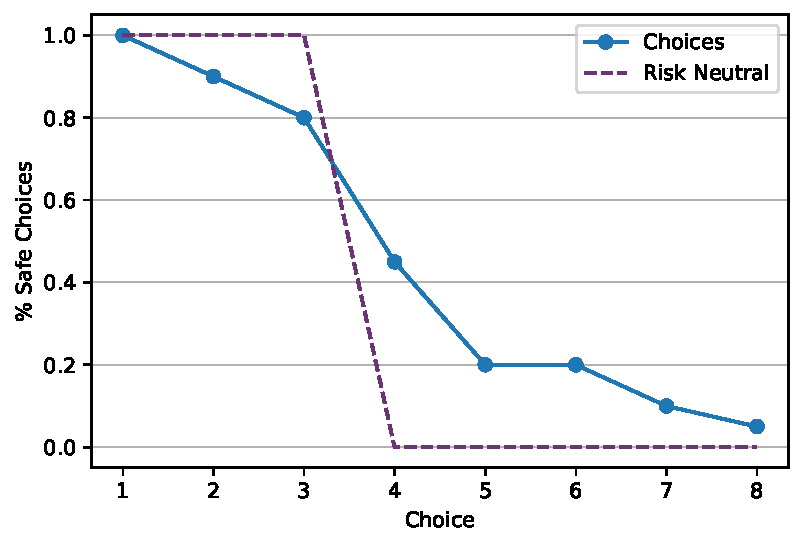
\includegraphics{graphics/aggregate_plot.pdf}
  \caption{Choices of participants versus perfectly risk neutral choices}
  \label{fig:choices}
\end{figure}

\subsection{Implementation}\label{sec:implementation}
The experiment was implemented in oTree \parencite{chen_otreeopen-source_2016}, which is an open-source framework for implementing economics experiments. It is based on Python and uses Django to create a front-end for users to participate in experiments. A graphical user interface for creating experiments exist in the oTree Studio. However, this experiment was entirely produced by applying techniques learned in the Programming Techniques course and additional self-study.

\textcite{holzmeister_otree_2017} made an implementation of the \cite{holt_risk_2002} MPL in oTree, which has been used as a resource in understanding how to implement a similar experiment in oTree. 


\subsection{Code}

oTree is developed with an object-oriented approach to encourage the efficient development of experiments. To develop experiments in oTree by writing Python code, one should have a fundamental understanding of how object-oriented programming works. 

The code for our project is available on GitHub\footnote{GitHub repository with installation instructions: \url{https://github.com/olafghanizadeh/hl_mpl}.}. In order to understand and explain what the code does, each line of code is commented according to the PEP 8 style guide. 



In our implementation of this experiment, we follow the recommendations stated in the oTree documentation and put most of our code in the \mintinline{python}{models.py} file of the project. The \mintinline{python}{pages.py} file contains our templating logic for the front-end, and we want to avoid doing calculations or computations in this file. We want to limit \mintinline{python}{pages.py} to defining forms for user input and making variables available to Django so that we can use them on our front-end. 

In the project, we used oTree's built-in classes extensively in order to structure the project properly and minimize code duplication. In oTree, each instance of an experiment is classified as a \mintinline{python}{Session}. Then, each part of the experiment is a \mintinline{python}{Subsession}. In each \mintinline{python}{Subsession} we have \mintinline{python}{Players} that go through the different \mintinline{python}{Pages}.

In our \mintinline{python}{models.py} file we utilized the \mintinline{python}{class Subsession} class and the \mintinline{python}{class Player} to construct our experiment. 

In \mintinline{python}{class Subsession}, we call the \mintinline{python}{creating_session} method to set the variables that will be the same for all the players in the experiment. In our code, we call the number of choices and the payoff multiplier from the session configuration and store them as session variables so that they can be referenced outside the scope of the \mintinline{python}{creating_session} method. The payoffs are loaded from the experiments Constants located in \mintinline{python}{config.py} where they are defined as a dictionary:

\begin{minted}{python}
 payoffs = {"A": [20, 16], "B": [38, 1]}
\end{minted}

In our experiment, the payoffs are multiplied by the multiplier defined in the session config. The multiplier was added to give the possibility of running experiments where they payoff is varying across subsessions to test for incentive effects as described in \cite{holt_risk_2002}. 

We then create the \mintinline{python}{index} variable by using list comprehension to create a list with integers corresponding to the number of choices in the lottery. We use this to create lists of probabilities and inverse probabilities in order to use in the drawing of the prize of the lottery, and to create lists of formatted probabilities to display to the user on the front-end. The following snippet of the code shows how we created a list corresponding to the number of choices in the game to aid in generating the forms that will be shown to the user. Finally, we create a list of tuples that contains the index, the form field name, and the probabilities for each choice and store it in a session variable so we can use it in our templates and other parts of the application.

\begin{minted}{python}
 form_fields = ['choice_' + str(k) for k in index]
 choices = list(zip(index, form_fields, formatted_p, formatted_inverse_p))
 self.session.vars['choices'] = choices
\end{minted}

The final thing we define in the \mintinline{python}{Subsession}-class for our experiment is the random drawing of which of the lottery choices to be chosen as the winning choice. This is then stored in participant variables that we can later call.

In \mintinline{python}{class Player(BasePlayer)}-class, we run all the code that should be run per player in the experiment. This is where you set the attributes of each player by registering form fields that are stored in the database. In our code, we have a field where the participant is asked to enter their name and their self-perceived preference for risks. oTree provides a multitude of different form field types in the form of widgets that can be used to build an experiment, but it is also possible to create custom widgets. 

We then create all the fields we need for the number of choices by using a \mintinline{python}{for} loop, as mentioned in the comments in the code it was necessary to use the \mintinline{python}{locals()} function to access the local scope of the application, a similar solution was used in the \cite{holzmeister_otree_2017} implementation. We define three additional attributes to store information about the outcome of the lottery. Lastly, we set the \mintinline{python}{set_payoffs} method in order to store the rewards for each player in the database. In our experiment, the payoff is randomly drawn based on a probability distribution in each choice. Therefore we need to run this for each player in this method. This was done using the \mintinline{python}{numpy.random.choice()} function, which draws $n$ random samples from a list, and it accepts a probability for each element in the list. To do this, we get the lists of probabilities that we stored in the session variables previously and concatenate them into one list where we can apply the NumPy function. We do the same with the payoffs stored as session variables to create a list of payoffs that NumPy can draw from. The application checks which option the player chose by accessing the relevant attribute in the Player object, executes the random draw and set the payoff for the player. One important thing to remember is that one has to call the \mintinline{python}{set_payoffs} in the desired place in the \mintinline{python}{Pages.py} file. In our case we call this method in the \mintinline{python}{before_next_page()} method on the results page. This implementation should be improved in a future version so that we can have an experiment with multiple rounds. 

\mintinline{python}{Pages.py} is mostly used to create the pages that the user will see, which in our project is the IntroPage, DecisionPage, and the ResultsPage, all of which were constructed by using the oTree Page class. In each page, we define which form fields we want to be displayed and which variables we want to expose for use in Django. One can also use the \mintinline{python}{vars_for_all_templates()} method to expose variables that are available across all templates. Each instance of the Page class allows an accompanying template in the templates folder where one can create the front-end with HTML and the Django Template Language. 


\subsection{Deployment}
The fact that oTree runs as a standalone web application that can be deployed to a web server are a massive advantage over closed-source solutions such as z-Tree. There is no need to install any software on the user side, making it easier to perform experiments on all types of devices and outside laboratory settings. 

Our project was deployed to Heroku, which is a Platform as a Service (PaaS) solution, in order to distribute it to the participants. It was done by using the tools made available through oTree Hub\footnote{Tool to aid Heroku deployments: \url{https://www.otreehub.com/}}. However, it is not necessary to use these tools once one has a good understanding of how the oTree production server and the Heroku deployment pipeline works. 

\subsection{Flask Application}
A simple Flask application was created to present the results during the class presentation. It uses d3.js to plot a version of Figure \ref{fig:choices}. The data was prepared with the help of pandas to create a JSON-like dictionary, which was then exported to the browser with the help of Flask's JSON utilities. The application was deployed to Heroku and is available at \href{https://progtech-flask-app.herokuapp.com/}{this link}. I was surprised at how simple it was to create a Flask application since one can use Python code directly, however, one should be aware of performance issues when working with large datasets and it would be better to export a cleaned dataset that was ready for presentation rather than doing the data preparation in the Flask application. 

\subsection{Future work}
Given that this project is a part of an introductory course in Python, it should be evident that the code has room for improvement. I would have liked to implement a custom class to generate a lottery with methods that could be called at the right places in oTree. This would have allowed for a more structured code with less duplication. It is possible that parts of this project will be used in actual experiments; however, that would warrant further testing of the code in order to make sure that it works as intended. It would also be useful to implement some new features to track additional data regarding the participant's interaction on the page. 


\newpage 
\section{Conclusion}
The project has been an excellent opportunity to apply skills learned in the course to an area in economics that interests me, and it has also presented me with an opportunity to apply the skills learned in my master thesis on an experimental economics research project. As explained in previous sections, there were limits to the results of the experiment; however, it gave a greater understanding of how an improved version could be implemented.



\newpage
\printbibliography

\end{document}







